% Chapter 1

\chapter{Stimulus Optimization for Neural Populations} % Main chapter title

\label{ch:optim} % For referencing the chapter elsewhere, use \ref{Chapter1} 

%----------------------------------------------------------------------------------------

% Define some commands to keep the formatting separated from the content 
\newcommand{\keyword}[1]{\textbf{#1}}


%------------------------------------------------------------------------------------

\section{Optimization}
Consider here, \textbf{EXAMPLE OF EASILY-UNDERSTANDIBLE OPTIMIZATION PROBLEM}. This example demonstrates that optimization, at the outset, is a simple problem. The complexity comes from large, high-dimensional data sets, and the plethora of approaches available. In this chapter, I will first describe the two main classes of optimization. Second, I will link these concepts to functional properties of neurons, focusing heavily on the visual system. I will then compare multiple algorithms when optimizing simulated neural data. 
\subsection*{What is Optimization?}
In its simplest form, optimization begins with an unknown function of inputs $\vec{x}$:
\begin{equation}
	f(\vec{x}) : \mathbb{R}^{n} \rightarrow \mathbb{R}
\end{equation}
where the output of the function is deterministic of it's inputs $\vec{x}$. The goal of optimization is to then find the set of inputs which minimizes (or maximizes) the output of the function $f(\vec{x})$. \textbf{MORE INTRO TO THIS SECTION BEFORE DERIVATIVES}

\subsection{Derivative-Based Optimization}
\label{sec:DerivB}
\textbf{MORE INTRO TO THIS SUBSECTION}
We an illustrate this using the simple example of a parabola. 
\begin{figure}
	\centering
	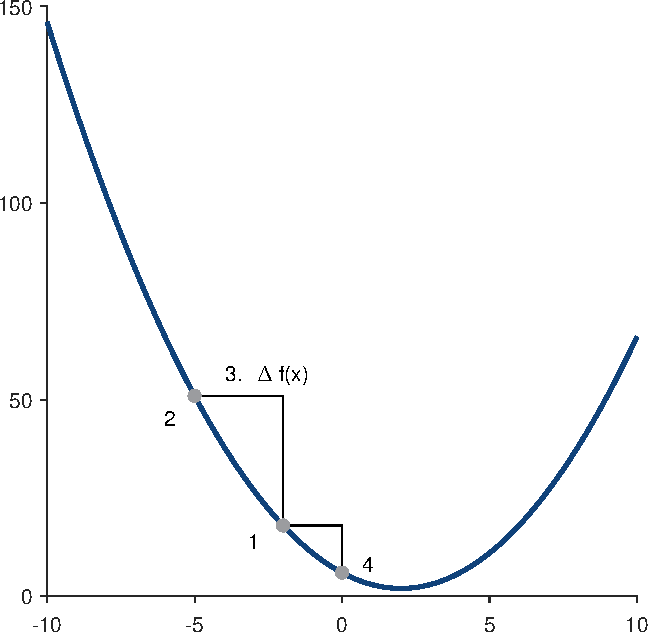
\includegraphics[width=86mm]{parabolaGradient.pdf}
	\caption{\textit{FigureTitle}}
	\label{fig:parabolaGradient}
\end{figure}
In the realm of low-noise and few variables, optimization is a rather simple problem of calculating the gradient and following it (Figure \ref{fig:parabolaGradient}). In Figure \ref{fig:parabolaGradient}, we test the function by using two random inputs (points 1\&2), calculate the gradient (3), and follow the gradient for the next input (4). This is an iterative process whereby each time we sample the function, we obtain more knowledge about it. Continuing this process will eventually result in $x=2$ as the global minimum. While this may appear obvious, in real world problems the blue line is unknown, necessitating the use of optimization techniques.
Unfortunately, because data is often high-noise and high-dimensional (in the parabola example there is only one input $x$, but most problems have many), calculating gradients quickly becomes computationally intractable in finite time. In addition to these constraints, real-world problems are often non-convex, meaning they have many local minima where gradient descent fails (\textbf{MAYBE NON-CONVEX FIGURE EXAMPLE}). This problem belies standard gradient approaches and lead to the development of Derivative-Free optimization techniques (see \ref{sec:DerivF}).

\subsection{Derivative-Free Optimization}
\label{sec:DerivF}
\subsection{Manifold Approximation with Particle Swarm (MAPS)}
\subsection{Genetic Algorithm}
genetic algorithm doesn't explore the radial dimension well. Even with a-priori knowledge of the proper radius, it doesn't do any better than MAPS because of this (prove it?).
\subsection{Bayesian estimation of true gradients?}
\subsection{Comparison across algorithms}

\section{Simulated Neural Population}
Assumptions:
\begin{enumerate}
	\item Peak FR$= 100 \frac{spk}{s}$
	\item Independent tuning to each feature dimension
	\item Deterministic responses (could fix)
	\item Independent Neurons
	\item Ground truth stimulus
\end{enumerate}

$x-pref$ is a matrix of euclidean distances for the current stimulus to each individual neurons' preferred stimulus. tuning is the neurons covariance matrix for the latent space (nLatents x nLatents). Diagonal is tuning width in that dimension and 0s off diagonal because feature tuning is assumed independent
\begin{equation}
someSymbol = -(x-pref)^T * tuning * (x-pref)
\end{equation}

response function: (come up with symbols for terms)
\begin{equation}
	\harpoon y = Peak * \exp{}
\end{equation}



%------------------------------------------------------------------------------------


 